\section{Problema 1}

\subsection{Análisis del algoritmo}

\indent La idea detrás de nuestra solución para el Problema 1 involucra recorrer
la lista de precios una sola vez. Logramos concluir que podíamos separar el
problema de la lista entera en sublistas disjuntas, donde un valor menor o igual
al minimo actual (inicializado en el primer elemento) marca el inicio de cada
una, ya que no nos interesa cuando un precio cualquiera precede a otro precio
inferior a él. De esta forma, creamos una variable que guarda la mejor ganancia
a medida que se va avanzando.
Dicha ganancia máxima empieza en 0 y se la pisa con la primer ganancia
calculada, que luego es pisada nuevamente por las ganancias mejores que ella en
caso de haberlas.\\
\\
\indent La ganancia se calcula de la siguiente forma:
\begin{itemize}
	\item Se setea la primera posición como posición de compra y de venta.
	\item En cada iteración se guarda la ganancia actual según el último
precio de compra y el precio de venta de esa posición.
	\item Se recorre el arreglo de precios y para cada posición, se mira si
su valor es mayor al máximo anterior, o menor al mínimo anterior.
Si es mayor, se toma como nuevo precio de venta $(max)$, y la resta entre el
precio de venta y el de compra es la ganancia de la sublista actual. Si es menor
$(min)$
indica el inicio de una sublista nueva. Se toma como nuevo precio de compra y se
guarda la ganancia en \textit{ganancia máxima} en caso de ser mayor que la
ganancia máxima anterior.
\end{itemize}

\indent Observación: Por comodidad, elegimos levantar los datos del archivo
$.in$
y pasarlos a un arreglo que es el que se le pasa a la función para resolver el
costo. En la sección complejidad podemos ver que encarar el ejercicio de esta
manera, no conlleva a una complejidad mayor a la requerida por la cátedra.\\

\indent La explicación anterior se puede ver reflejada en el siguiente
\textbf{Pseudocódigo}:

\begin{algorithm}
\caption{buscarGanancia (\textbf{in} precios: \textsl{int[]}) $\rightarrow$ res:
\textsl{int}}
\begin{algorithmic}[1]
\STATE $min \leftarrow precios[0], max \leftarrow precios[0]$

\FOR{$i = 1$ \textbf{to} $cantDias$}
	\IF{$precios[i] < min$}
		\STATE $min \leftarrow precios[i]$
		\STATE $max \leftarrow precios[i]$
	\ENDIF
	\IF{$precios[i] > max$}
		\STATE $max \leftarrow precios[i]$
	\ENDIF	
	\STATE $gananciaActual \leftarrow max - min$
	\IF{$gananciaActual > gananciaMax$}
		\STATE $gananciaMax \leftarrow gananciaActual$
	\ENDIF
\ENDFOR
\RETURN $gananciaMax$
\end{algorithmic}
\end{algorithm}

\clearpage

\subsection{Demostración de Correctitud}
\indent Para analizar la correctitud de nuestro algoritmo, queremos ver un caso
a modo de ejemplo:

\begin{figure}[h]
\centering                                                       
        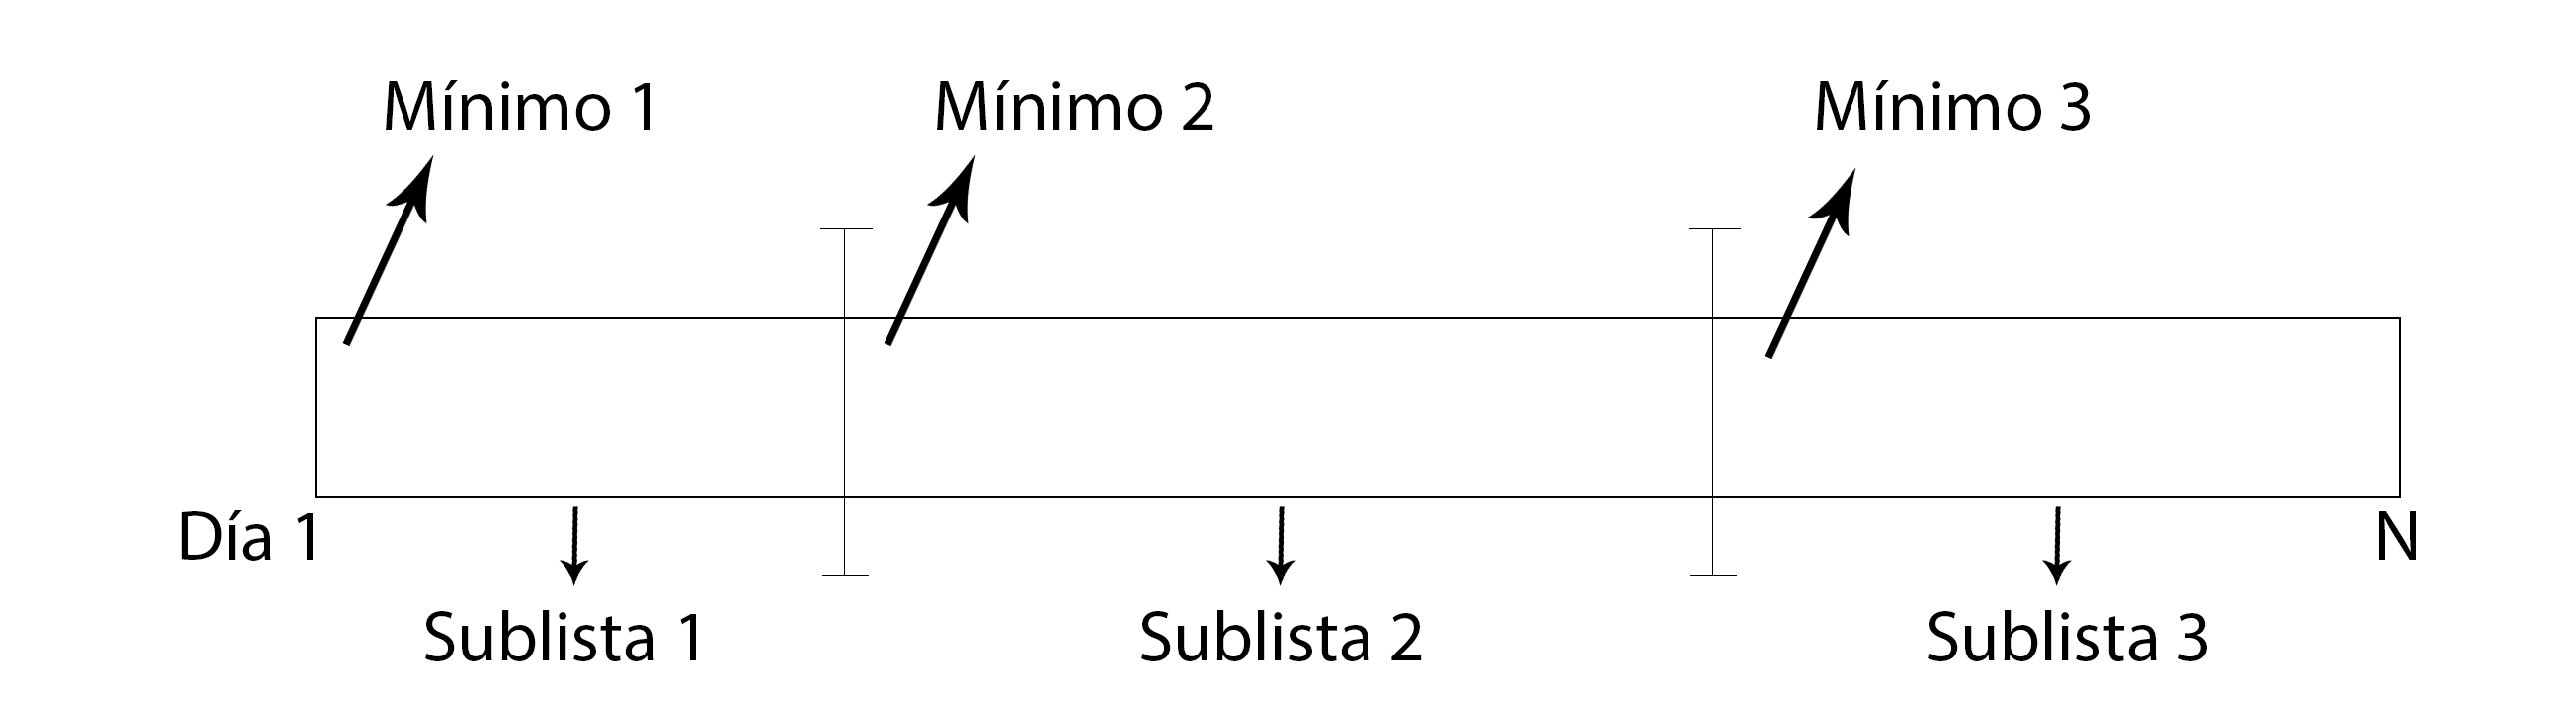
\includegraphics[width=300pt]{./figs/sublistas.png}
	\caption{Ejemplo con 3 mínimos}
	\label{fig:sublistas}
\end{figure}

\indent En la Figura ~\ref{fig:sublistas} podemos observar como los mínimos 1, 2
y 3 dividen al
arreglo original en 3 sublistas. Estos valores cumplen la relación:
$minimo 1$ $>$ $minimo 2$ $>$ $minimo3$. Cada una de las sublistas va a tener un
valor máximo, y por ende, una ganancia máxima. La ganancia máxima final va a ser
la mayor de las 3 ganancias máximas de cada una de las sublistas.\\

\indent Podemos ahora ver el caso general:\\
\indent Suponemos que hay un conjunto de $m$ índices en el arreglo, con $m$
$\leq$ $n$, tales que 
\begin{center}
 $precios[m_i]$ $>$ $precios[m_j]$ $\forall$ $m_i$ $<$ $m_j$ 
\end{center}
Esto quiere decir que tenemos $m$ mínimos y $m_0$ representa al primer mínimo,
osea el primer elemento del arreglo. Esto quiere decir que vamos a tener el
arreglo partido en $m$ sublistas.\\
\indent Queremos ver que dividir en estas sublistas es correcto y que
efectivamente se encuentra la mayor ganancia en el arreglo. Para esto vamos a
tomar el caso particular de una sublista que empieza en el índice $m_i$ y
termina en el índice $m_{i+1}$ del arreglo. Como dijimos anteriormente hay un
valor máximo en esa sublista ($max_1$), por lo que la ganancia máxima de esa
sublista particular es $max_1$ -  $precios[m_i]$. Ahora bien, si dado un índice
mayor a $m_{i+1}$ encontramos un valor $max_2$, que cumple $max_2$ $>$ $max_1$
vamos a calcular una nueva ganancia. Vemos que esta ganancia podría ser:
\begin{center}
 Ganancia1 = $max_2$ -  $precios[m_i]$\\
 o bien\\
 Ganancia2 = $max_2$ -  $precios[m_{i+1}]$\\
\end{center}
\indent Pero como vimos que $precios[m_{i+1}]$ $<$ $precios[m_i]$ vale que:
\begin{center}
 Ganancia1 $<$ Ganancia2
\end{center}
\indent Y esto demuestra que una vez que se encuentra un nuevo mínimo, esta bien
guardar el mejor valor de ganancia hasta el momento y actualizar el mínimo al
nuevo valor para seguir buscando una ganancia mayor y que efectivamente la
variable $gananciaMax$ contiene la mayor ganancia que se puede obtener de los
precios pasados como parametro.\\
\indent Como no hay algún caso que no hayamos contemplado, podemos concluir que
nuestro algoritmo es correcto.




\clearpage
\subsection{Complejidad}
\indent Antes de analizar la complejidad del algoritmo en si, analizaremos la
complejidad de crear el arreglo para resolver el problema. Según la
documentación de $Java$ pudimos observar que se puede crear un arreglo en $O(n)$
(en nuestro caso $n$ va a ser el tamaño de entrada)
e indexar sus posiciones en $O(1)$. Teniendo en cuenta esto, podemos ver que el
costo de crear un arreglo vacío mas el costo de llenarlo con los valores que
queremos es $O(n)$ + $O(n)$ = $O(2n)$ que por el álgebra de ordenes es $O(n)$.\\
\indent Básicamente, nuestro algoritmo recorre linealmente el arreglo de los
días y va guardando la ganancia máxima, que luego es el valor devuelto.\\
\indent Para empezar a analizar la complejidad, podemos notar que ciclamos por
todas las posiciones del arreglo una sola vez. Esto quiere decir que la
complejidad que tenemos va a ser de $O(n)$ por el costo del cuerpo del $for$,
\textbf{considerando a n, como el tamaño del arreglo (cantidad de días).}\\
\indent Una vez analizado el ciclo, podemos meternos de lleno con el cuerpo del
mismo y ver que es lo que pasa adentro.\\
\indent Tenemos 3 comparaciones y varias asignaciones para tener en cuenta su
complejidad. Para ver el costo de estas operaciones recurrimos a la
documentación de $Java$ y comprobamos que tanto las comparaciones de enteros,
como las indexaciones en arreglos, toman un tiempo constante. Visto esto,
podemos analizar el peor caso del cuerpo del ciclo. Tenemos 2 casos disjuntos a
tener en cuenta:

\begin{itemize}
 \item precios[i] $<$ min: el valor del precio del producto en el día $i$ es
menor al mínimo anterior.
 \item precios[i] $>$ max: el valor del precio del producto en el día $i$ es
mayor al máximo anterior.
\end{itemize}

\indent Si ninguno de los casos anteriores se cumple, es porque el precio de ese
día no va a influir en la ganancia final, por lo que no es un caso interesante
para analizar en la complejidad.\\
\indent Se puede ver claramente que estos casos son disjuntos porque al comparar
por menor y mayor (nunca por igual) no puede pasar que un numero cumpla ambas
condiciones.\\
\indent La comparación por menor al mínimo, lleva a tener que hacer 2
indexaciones en el arreglo y 2 asignaciones de enteros, cuando la comparación de
mayor al máximo lleva a tener 1 sola indexación y una asignación, aunque también
al cambiar el máximo valor, ahora vamos a tener una mayor ganancia, por lo que
sumamos otra asignación mas. Por lo tanto
consideramos el peor caso, como un arreglo estrictamente decreciente, adonde se
cumple siempre la guarda del primer $if$, aunque no es muy distinto de un caso
creciente, por lo que consideramos que son semejantes en complejidad y no hay un
caso que sea mucho peor que el otro. Como estamos usando el modelo
uniforme, en este caso tenemos $O(1)$ + $O(1)$ + $O(1)$ + $O(1)$ que por el
álgebra de ordenes, es $O(1)$. \\                                               
\indent Luego hacemos una resta entre 2 enteros, nuevamente $O(1)$ y otra
asignación. Si se cumple la guarda del ultimo $if$, nuevamente hacemos una
comparación y una asignación, por lo tanto seguimos trabajando en tiempo
constante.\\
\indent Por lo visto anteriormente, podemos decir que la complejidad del cuerpo
del ciclo es $O(1)$ y como este ciclo se ejecuta $n$ veces, concluimos que la
complejidad total del ciclo es $O(n)$. Ahora bien, si sumamos la complejidad de
crear el arreglo, mas la de resolverlo, tenemos: $O(n)$ + $O(n)$ = $O(2n)$ que
por el álgebra de ordenes es $O(n)$.\\
\indent \textbf{Por lo tanto concluimos que la complejidad del algoritmo es
$O(n)$}.\\

\clearpage

\subsection{Análisis del tiempo de ejecución}

\indent Para tomar los tiempos de este algoritmo, consideramos 3 tipos de casos
de prueba. Para cada uno de los casos, generamos tests variando de a 500 el
tamaño de entrada (cantidad de días), hasta 15000.

\begin{itemize}
 \item Caso Creciente: Números estrictamente crecientes.
 \item Caso Decreciente: Números estrictamente decrecientes.
 \item Caso Random: Para generar un caso que se relacione con la vida real,
realizamos un algoritmo adonde el precio varia según el resultado de un
random. Nuestro algoritmo que genera el caso, realiza un random para el valor
del producto en el primer día y luego para cada nuevo día realiza otro random
cuyo resultado sera 0 o 1. En el caso de que sea 0, el precio del producto se
incrementa en 1. En el caso contrario, el precio del producto se decrementa en
1. Una salvedad respecto a este caso es que aquí tomamos la decisión de que cada
instancia del caso contuviera a la anterior. Esta decisión fue
tomada para mantener la uniformidad del set de de días, lo cual se daba
naturalmente en los casos
anteriores porque había una relación de orden estricta.\footnote{Para ver mas
detalles del algoritmo referirse a la carpeta
testsAvanzados.}
\end{itemize}

\indent Para cada instancia de cada caso realizamos 1000 iteraciones, eliminamos
outliers que distaban un 10\% del promedio de los datos y nos quedamos con el
máximo tiempo entre todas las iteraciones
restantes.\\
\indent Los resultados obtenidos se pueden ver reflejados en el
siguiente gráfico:

\begin{figure}[h]
\centering                                                       
        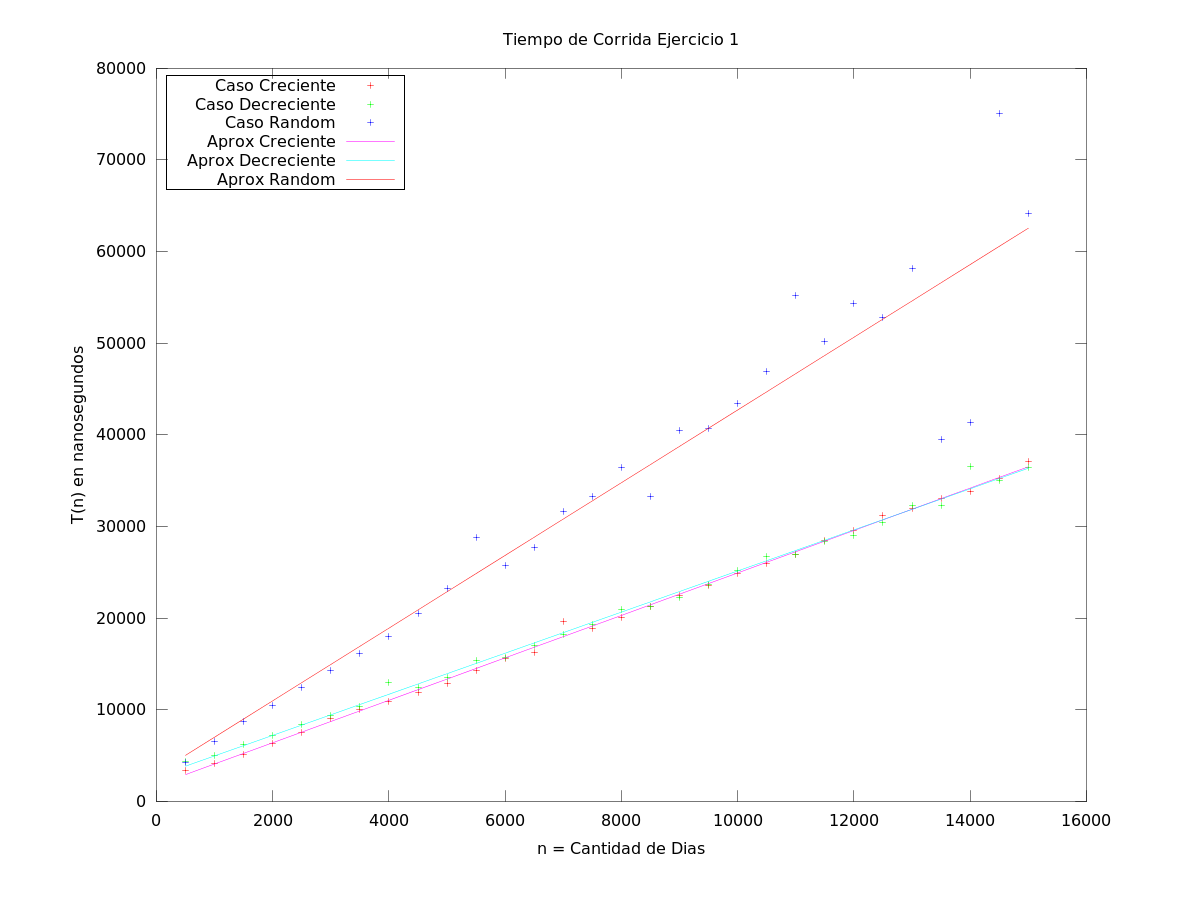
\includegraphics[width=420pt]{./figs/ej1.png}
	\caption{Gráfico del tiempo de corrida de los tests.}
	\label{fig:p1tiempos}
\end{figure}


\indent Analizando el Gráfico de la Figura ~\ref{fig:p1tiempos}, podemos
comprobar los resultados que expresamos en la sección de complejidad. Se ve que
los tiempos tienen un comportamiento lineal como el esperado y también podemos
observar como los casos Decreciente y Creciente tienen un comportamiento muy
similar, como era de esperarse.\\

\clearpage

\indent Ahora bien, si miramos el caso Random, nos encontramos con una
particularidad. Para poder analizarla, nos ayudamos del siguiente gráfico:

\begin{figure}[h]
\centering                                                       
        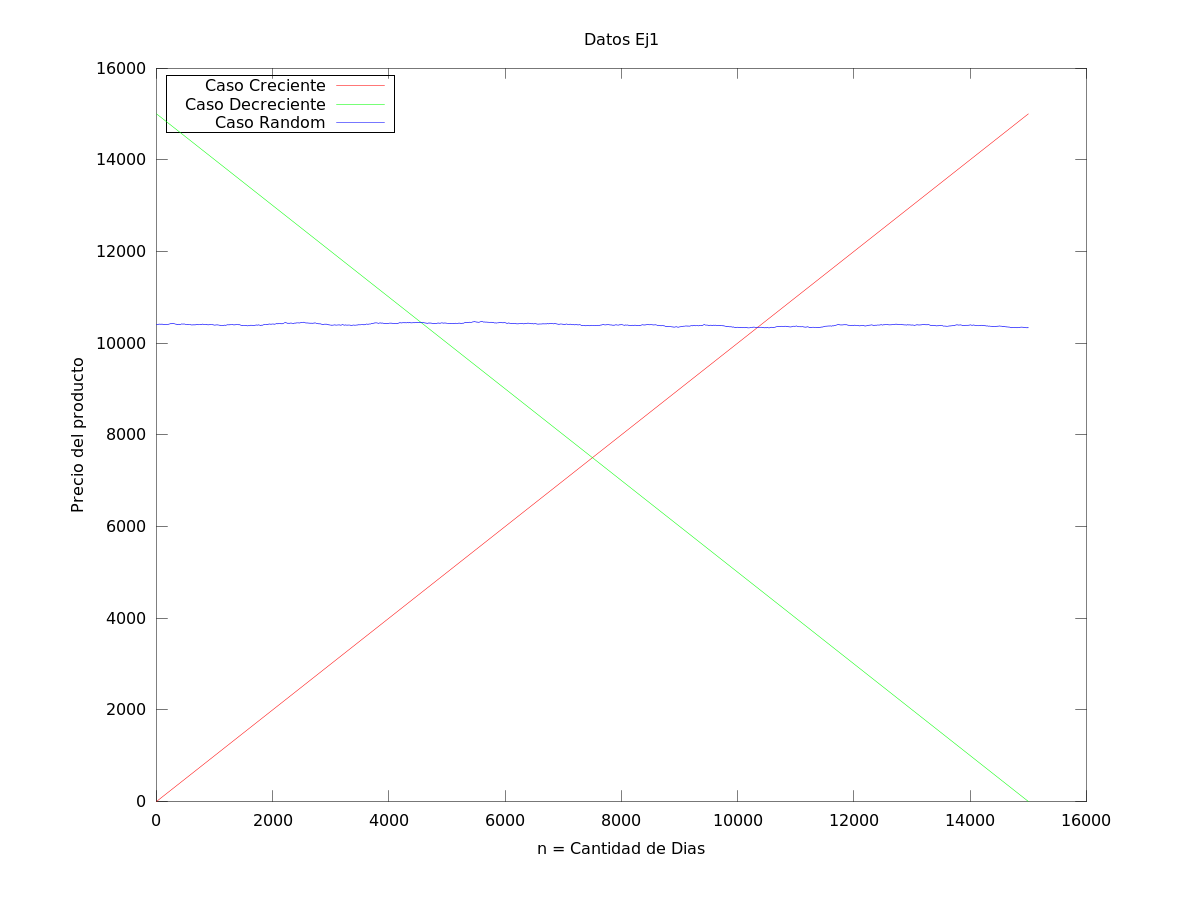
\includegraphics[width=420pt]{./figs/dataej1.png}
	\caption{Gráfico de los datos utilizados para los tests.}
	\label{fig:p1data}
\end{figure}

\indent En la Figura ~\ref{fig:p1data} podemos observar los valores con los que
fueron corridos cada uno de los casos. Podemos observar como los datos de los
casos Crecientes y Decrecientes, tienen una distribución lineal, mientras que
los del caso Random tienen una distribución mas bien constante.\\
\indent En la Figura ~\ref{fig:p1tiempos} podemos observar como los tiempos son
lineales y entre los casos Creciente y Decreciente la diferencia radica en una
minima diferencia en el valor de la constante que acompaña al termino lineal.
Ahora bien, podemos también ver que el caso Random también es lineal, pero con
una constante mayor a la de los casos anteriores.\\
\indent De estos resultados podemos concluir que mientras los casos Creciente y
Decreciente realizan siempre la misma operación (actualizar mínimo o máximo,
pero nunca las 2 en una misma corrida), el caso Random fuerza al algoritmo a
hacer actualizaciones de mínimo y máximo sin un patrón definido y por esta
particularidad creemos que los tiempos de corrida son superiores.\\











